\documentclass[a4paper, fontsize=11pt]{article}

\usepackage{graphicx}
\usepackage{amsmath,amsfonts,amsthm} % Math packages
\usepackage[english]{babel} % English language/hyphenation
\usepackage[colorlinks=true,linkcolor=black, urlcolor=blue,
citecolor=blue]{hyperref}


\author{Audun Tahina Reitan}
\title{Studies of phase transitions in magnetic systems}

\begin{document}
\maketitle

\section{Abstract}
Study of the square-lattice Ising model and reaching the most likely state. Also an study of the critical temperature for spontaneous magnetization for different resolutions of the model.

\section{Introduction}
In this project we will study the square-lattice Ising model in two dimensions, with the simplest form for the energy with, i.e.\ without an externally applied magnetic field. The Ising model is a model to simulate phase transitions in an canonical ensemble, where on each lattice site the objects can only have binary values (for example 0 and 1 or 1 and -1). The project will use 1 and -1 as the binary values for spin pointing up or down respectively. The expression for the energy becomes in this case:

\begin{equation} \label{eq:1}
E = -J \sum_{<kl>}^N s_k s_l, \hspace{5mm} s_i = \pm 1
\end{equation}

\noindent
with $J$ as the coupling constant and $s_k$ is the spin of a lattice point and $<kl>$ means that the summation is over nearest neighbors only.

We will assume periodic boundary conditions for the lattice, which means whenever a lattice point at the boundary needs an adjacent point for computation and there is none, the opposite point in the same dimension will be used.

The project will study the if the Monte Carlo simulation reaches the most likely state and study if the implementation gets the critical temperature for spontaneous magnetization correctly.

\section{Methods} \label{mathrefs}
\subsection{Implementation}

The code for this project is implemented at \url{https://github.com/auduntre/FYS4150-1/tree/master/project4}. This is the GitHub repo referenced throughout the project.

This code for this project based upon the code for Monte Carlo simulation using the Metropolis algorithm given in the FYS-3150 github repo: \cite{fys4150}. An explanation for the Metropolis algorithm can be found in \cite[p. 404-405]{Hjort-Jensen}. Otherwise  check the github repo for documentation and explanation of the code.

The parallelization is achieved by dividing of the temperature steps between each process using MPI for speeding up the computation.

This code is written in cooperation with Marius Holm which has github repo: \url{https://github.com/MariusHolm}. 

\subsection{Analytical verification of the model}
To verify the implementation, comparison to an know analytical solution is of great use. Assuming we have only two spins in each dimension ($L=2$) we can find the analytical expression for the partition function. The partition function in an canonical ensemble is:

\begin{equation} \label{eq:2}
Z = \sum_{i=1}^{M}e^{-\beta E_i},
\end{equation}

\noindent
where $M$ is all the micro-states, $\beta = \frac{1}{kT}$ with $k$ being the Boltzmann constant and $T$ is temperature, and $E_i$ is the energy for a micro-state $i$  \cite[p. 422]{Hjort-Jensen}. The formula for energy $E_i$ is given by (\ref{eq:1}).

In a two by two square lattice there will be 16 different micro-states. An example of the energy calculated is given here for a lattice with all spin up:

\begin{equation}
\begin{split}
E_0 & = - J \left(1^2 + 1^2 + 1^2 + 1^2 + 1^2 + 1^2 + 1^2 + 1^2 + 1^2 \right) \\
    & =  -8J.
\end{split}
\end{equation}

The degeneracy, $\Omega(E_0)$, of this configuration is $1$ since there is only one way to have 4 spins up in a 2x2 lattice. The magnetization $\mathcal{M}$ can simply be measured as the sum of spins in the lattice \cite[p. 423]{Hjort-Jensen}.

\begin{equation}
\mathcal{M}_i = \sum_k^N s_k.
\end{equation}

From \cite[p. 424]{Hjort-Jensen} we get a table with possible configurations of the energy and number of degeneracy for a certain number of spins:

\begin{center}
\begin{tabular}{cccr}
\hline \\
Spins Up 	& $\Omega(E_0)$ 	& $E_i$ 	& $M_i$ \\
\hline \\
$4$ 	& $1$	& $-8J$		& $4$ \\
$3$ 	& $4$	& $0$		& $2$ \\
$2$ 	& $4$	& $0$		& $0$ \\
$2$ 	& $2$	& $8J$		& $0$ \\
$1$ 	& $4$	& $0$		& $-2$ \\
$0$ 	& $1$	& $-8J$		& $-4$ \\
\hline \\
\end{tabular}
\end{center}

Using this we find the solution for the partition function:

\begin{equation}
\begin{split}
Z &= 1e^{8J\beta} + 4e^{- 0 \cdot \beta} + 4e^{- 0 \cdot \beta} + 2e^{- 8J \beta } + 4e^{- 0 \cdot \beta} + 1e^{ 8J \beta} \\
  &= 2e^{8J \beta } + 2e^{- 8J \beta} + 12 \\
  &= 4 \cosh{(8J \beta)} + 12
\end{split}
\end{equation}

Using the partition function we can now find the analytical values for the expectation of energy $\left< E \right>$, the mean magnetization $\left< |\mathcal{M}| \right>$, the specific heat $C_v$ and the susceptibility $\mathcal{X}$ as functions of the temperature $T$. The probability distribution for the canonical ensemble is given as $P_i(\beta) = \frac{1}{Z}e^{-\beta E_i}$ \cite[p. 420]{Hjort-Jensen}.


\begin{equation}
\left< E \right> = \sum_{i=1}^{M} E_i P_i (\beta) = \frac{1}{Z} \sum_{i=1}^{M} E_i e^{-\beta E_i} = - \frac{J}{Z} \left(16e^{8J \beta} - 16e^{-8J \beta}\right)
\end{equation}

\begin{equation}
\begin{split}
\left< E^2 \right> &= \sum_{i=1}^{M} E^2_i P_i (\beta) = \frac{1}{Z} \sum_{i=1}^{M} E^2_i e^{-\beta E_i} = \frac{J^2}{Z} \left(2 \cdot 64e^{8J \beta} - 2 \cdot 64e^{-8J \beta}\right) \\
&= \frac{J^2}{Z} \left(128e^{8J \beta} - 128e^{-8J \beta} \right)
\end{split}
\end{equation}

The variance of energy $\sigma_{E}$ is:

\begin{equation}
\sigma_{E} = \left< E^2 \right> - \left< E \right>^2
\end{equation}

\begin{equation}
C_v = \frac{\sigma_{E}}{kT}
\end{equation}

\begin{equation}
\begin{split}
\left<|\mathcal{M}| \right> &= \sum_{i=1}^{M} \mathcal{M}_i P_i (\beta) = \frac{1}{Z} \sum_{i=1}^{M} \mathcal{M}_i e^{-\beta E_i} \\
&= \frac{1}{Z} \left(1 \cdot 4e^{8J \beta} + 4 \cdot 2 + 4 \cdot 2 + 1 \cdot 4e^{8J \beta} \right) \\
&= \frac{1}{Z} \left(8e^{8J \beta} + 16\right)
\end{split} 
\end{equation}

\begin{equation}
\begin{split}
\left<\mathcal{M} \right> &= \sum_{i=1}^{M} \mathcal{M}_i P_i (\beta) = \frac{1}{Z} \sum_{i=1}^{M} \mathcal{M}_i e^{-\beta E_i} \\
&= \frac{1}{Z} \left(1 \cdot 4e^{8J \beta} + 4 \cdot 2 + 4 \cdot (-2) + 1 \cdot (-4)e^{8J \beta} \right) \\
&= 0
\end{split}
\end{equation}

\begin{equation}
\begin{split}
\left<\mathcal{M}^2 \right> &= \sum_{i=1}^{M} \mathcal{M}^2_i P_i (\beta) = \frac{1}{Z} \sum_{i=1}^{M} \mathcal{M}^2_i e^{-\beta E_i} \\
&= \frac{1}{Z} \left( 1 \cdot 16e^{8J \beta} + 4 \cdot 4 + 4 \cdot 4 + 1 \cdot 16e^{8J \beta} \right) \\
&= \frac{1}{Z} \left(32e^{8J \beta}  + 32\right)
\end{split}
\end{equation}

The variance of magnetization is $\sigma_{\mathcal{M}}$:

\begin{equation}
\sigma_{\mathcal{M}} = \left<\mathcal{M}^2 \right> - \left<\mathcal{M} \right>^2 = \frac{1}{Z} \left(32e^{8J \beta}  + 32\right),
\end{equation}

so the susceptibility becomes:


\begin{equation}
\mathcal{X} = \frac{O_{\mathcal{M}}}{kT} = \frac{\left(32e^{8J \beta}  + 32\right)}{Z}\beta
\end{equation}

Now to verify the implementation we set the temperature to $T = 1$ in units $(kT/J)$. $N = 4$ is the number of spins in the 2x2 lattice. Running the \verb+ising_model+ for a different amount of Monte Carlo Cycles:

\begin{center}
\begin{tabular}{ccccc}
\hline \\
Monte Carlo Cycles	& $E/N$  & $C_v/N$ & $\mathcal{X}/N$ & $|\mathcal{M}|/N$ \\
\hline \\
1000 	& -1.9980e+00  & 1.5984e-02  & 9.9900e-04  & 9.9950e-01 \\
10000  	& -1.9962      & 0.03034224  & 3.7022397   & 0.99855 \\
100000  & -1.99644     & 0.02842931  & 3.8239065   & 0.998865 \\
1000000 & -1.996112    & 0.03104353  & 3.991801    & 0.9987165 \\
10000000  & -1.9959112 & 0.03264353  & 3.9927068   & 0.9986386 \\
\hline \\
Analytical & -1.99598209 & 0.03208233  &3.99330378  &1.00334778 \\
\hline
\end{tabular}
\end{center}

We see that you need up to 1 million MCCs to get achieve a good agreement with the analytical solutions.

\subsection{Parallelization}
Timing the parallelized code with different amount of processes for $L = 40$, temperature $T \in [2.0, 3.0]$ with temperature step $\Delta T = 0.05$ and 10,000 MCCs and comparing it to the serial code:

\begin{center}
\begin{tabular}{ccc}
\hline \\
Processes &Time [s] & $\approx$ Speed up \\
\hline \\
1 &16.83  &1.00\\
2 &8.46 &1.99 \\
4 &4.44 &3.79 \\
8 &2.52 &6.67 \\
16 &1.83 &9.19\\
\hline \\
Serial &16.82 & 1.00 \\
\hline \\
\end{tabular}
\end{center}

The speed-up is substantially when more temperature steps is included due to the way the code is implemented (parallelized in temperature steps).

\section{Results}
\subsection{Most likely state}
Analyzing the time in MCCs it takes for the square lattice of $L = 20$ to achieve the equilibrium situation for temperatures of $T = 1$ and $T = 2.4$ in units $(kT/J)$.

\begin{center}
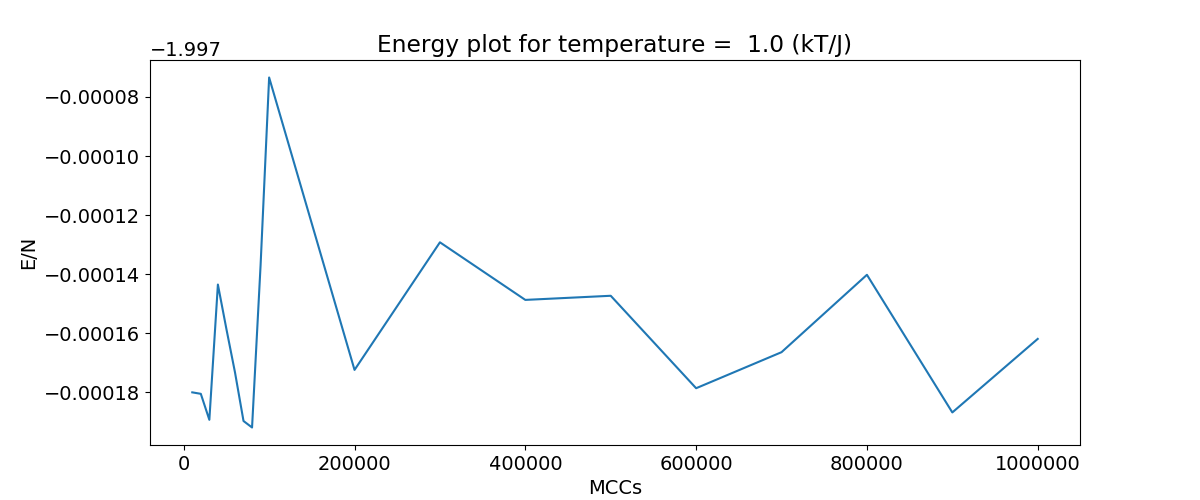
\includegraphics[scale=0.45]{ET1.png} 
\end{center}

\begin{center}
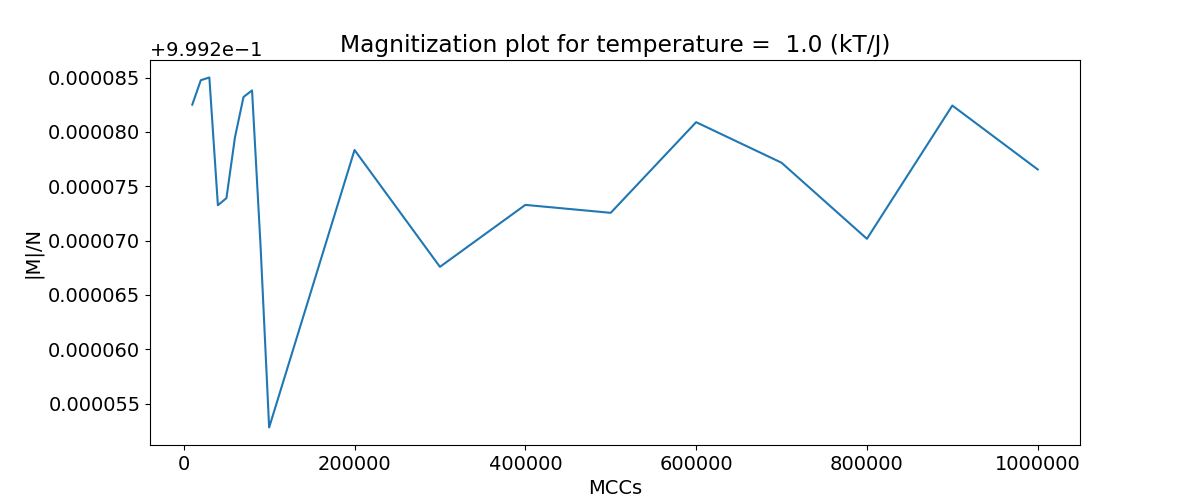
\includegraphics[scale=0.45]{MT1.png} 
\end{center}

\begin{center}
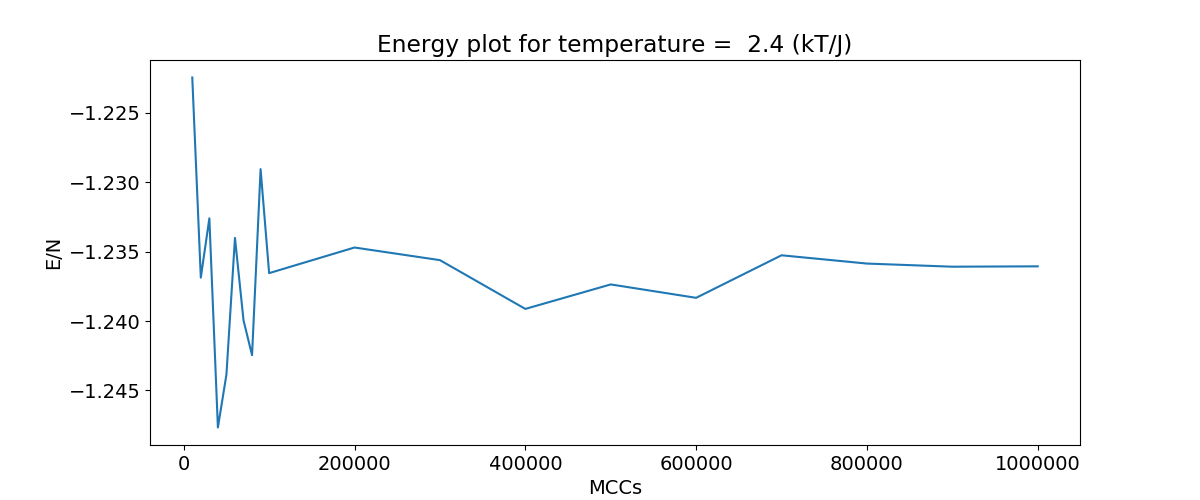
\includegraphics[scale=0.45]{ET24.png} 
\end{center}

\begin{center}
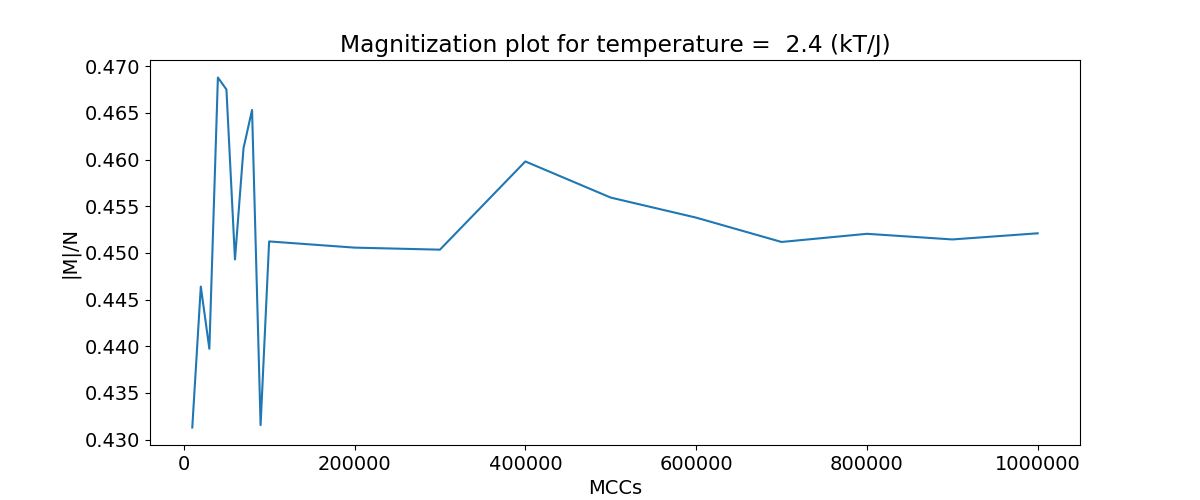
\includegraphics[scale=0.45]{MT24.png} 
\end{center}

For $T = 2.4$ the system seem to have reached an equilibrium situation around 100,000 MCCs where the value for magnetization and energy are not so volatile with increasing MCCs. This seems like a fine estimation for an equilibration time. The values for $T = 1$ are much more volatile, but already around 200,000 MCCs the graphs seems to be oscillating less with increasing MCCs.

\subsection{Analyzing the probability distribution}
Se github repo in the scripts folder for analyzation of the probability distribution after reaching the most likely state. The file in question is the jupyter notebook \verb+pdf.ipynb+.

\subsection{Numerical study of phase transitions}
Studying the the temperature space of $T \in [2.0 2.5]$.

\begin{center}
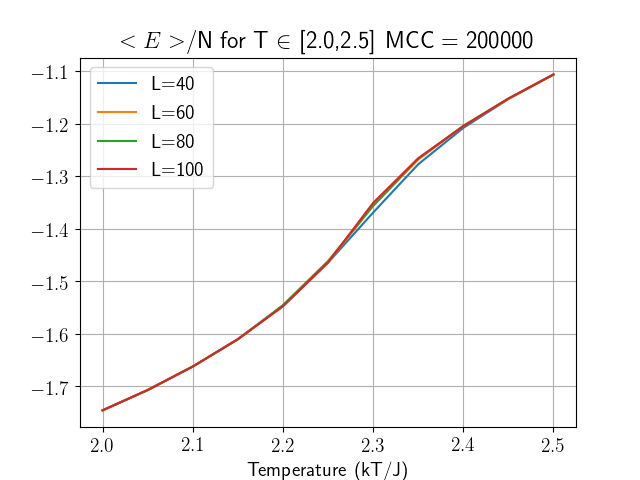
\includegraphics[scale=0.7]{p1.png} 
\end{center}

\begin{center}
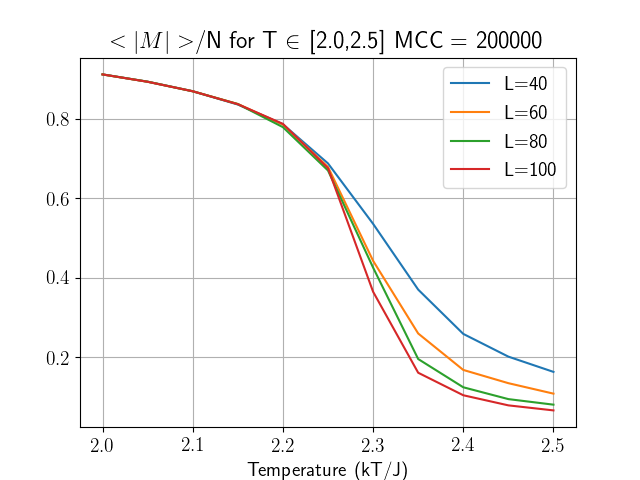
\includegraphics[scale=0.7]{p2.png} 
\end{center}

\begin{center}
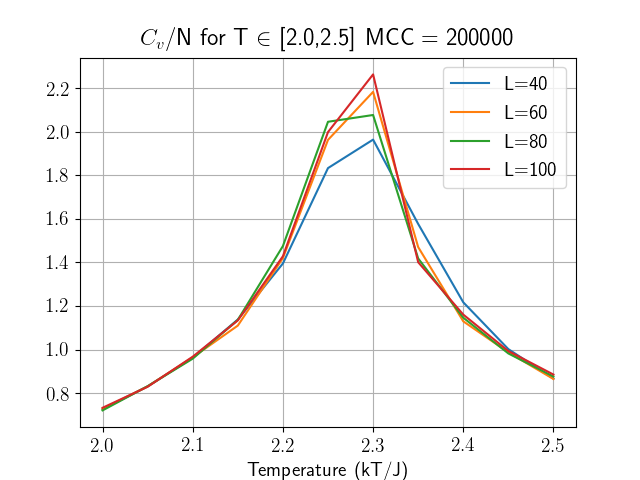
\includegraphics[scale=0.7]{p3.png} 
\end{center}

\begin{center}
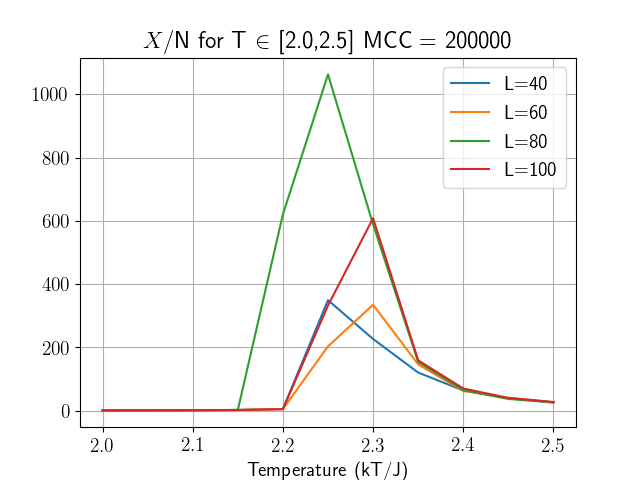
\includegraphics[scale=0.7]{p4.png} 
\end{center}

Analyzing the graphs it's clear there is a phase transition in the neighborhood $2.2 < T < 2.3$. The mean of the magnetization goes from close to zero for temperature over $2.3$ to trending towards $1$ under $2.2$. The critical temperature for the Ising model, where it spontaneously becomes ferromagnetic, must therefore be in this interval. The susceptibility and the specific heat also spikes in this area also indicating a phase change here.


\section{Conclusions}
The project have shown that Monte Carlo simulations using the Metropolis Algorithm for the square-lattice Ising model reaches the equilibrium state, even though it requires long computation time with MCCs $ > 100,000$ for the small case when $L = 20$. Parallelization offers an huge speed up which can migrate most of the time required.


Studying the case with increasing L $\rightarrow \infty$ we see that the model approaches the exact values for the critical temperature for the Ising model which is $\approx 2.269$ \cite{Hjort-Jensen}.


\bibliographystyle{apalike}
\bibliography{references}

\end{document}